
\subsection{Paquetes}
  \index{Paquete}
  
  De la misma forma en que un computador se organiza en carpetas, un proyecto se organiza en 
  paquetes.

  El principal objetivo de los paquetes es darle organización a nuestro código, porque, al igual 
  que tener una carpeta repleta de archivos (te estoy mirando a ti que tienes el escritorio 
  tapizado en íconos), tener todo el código de nuestra aplicación en una carpeta (o en el mismo 
  archivo \texttt{D:}) es barbarie.

  La gracia de usar paquetes en vez de simplemente carpetas es que podemos incorporar la lógica de
  los paquetes en nuestro código.
  Además, si se utilizan correctamente podemos evitar gran parte de los problemas que podrían
  surgir al momento de interactuar con librerías externas.

  \textit{Kotlin} (al igual que \textit{Java} y \textit{Scala}) permiten organizar nuestro código 
  en paquetes, mientras que otros lenguajes como \textit{Python} y \textit{C++} 
  no.\footnote{En lugar de paquetes \textit{Python} provee módulos y \textit{C++} tiene 
  \textit{namespaces}, ambas cumplen los mismos objetivos que los paquetes, pero se utilizan de 
  forma distinta. 
  Es importante informarse de esas diferencias cuando están aprendiendo un nuevo lenguaje.}
  El estándar para nombrar paquetes es el mismo para \textit{Java}, \textit{Kotlin} y 
  \textit{Scala}: 
  \begin{itemize}
    \item El nombre del paquete debe ser único (se recomienda usar el dominio de la empresa o 
      persona que lo creó).
    \item El nombre del paquete debe ser escrito en minúsculas.
    \item El nombre del paquete no debe incluir guiones bajos (\texttt{\_}).
    \item El nombre del paquete puede incluir guiones (\texttt{-}), pero no se recomienda.
  \end{itemize}

  Veamos algunos ejemplos:

  \begin{kotlin}
    package cl.ravenhill.intellij.basics; // Bien
    package cl.ravenhill.intelliJBasics; // Mal, el nombre no debe incluir mayúsculas
    package cl.ravenhill.intellij_basics; // Mal, el nombre no debe incluir guiones bajos
    package cl.ravenhill.intellij-basics; // Permitido, pero no recomendado
  \end{kotlin}

  Busquemos la carpeta \texttt{src/main/kotlin} y creemos un paquete llamado 
  \url{cl.ravenhill.intellij.basics} haciendo click derecho sobre la carpeta \texttt{kotlin} y 
  seleccionando \textit{New} \texttt{->} \textit{Package}.

  \begin{figure}[ht!]
    \centering
    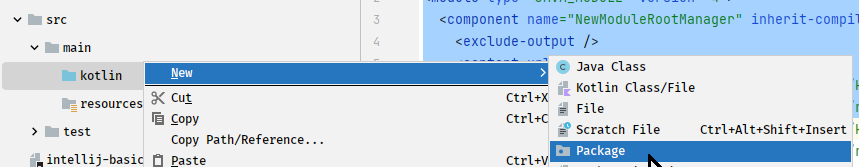
\includegraphics[width=0.8\textwidth]{img/Por_algo_se_empieza/idea64_new_package.png}
    \caption{Creando un nuevo paquete}
    \label{fig:idea64_new_package}
  \end{figure}

  Es importante acostumbrarse a crear paquetes para organizar el código por dos razones:
  \begin{itemize}
    \item Siempre que se trabaje con librerías externas, es muy probable que se encuentren con 
      paquetes que no son de su propiedad, y que no pueden modificar.
    \item Cuando una aplicación crece, los paquetes nos permiten organizar el código de forma 
      lógica.
  \end{itemize}